\documentclass{beamer}

%\usepackage[utf8x]{inputenc}
\usepackage{textcomp}
%\usepackage{graphicx}
%\usepackage{subcaption}
%\usepackage{floatrow}
\usepackage{subfig}
\usepackage{array}

\definecolor{OSUdkbrn}{RGB}{104,80,64}
\definecolor{OSUmedbrn}{RGB}{176,96,16}
\definecolor{OSUltbrn}{RGB}{224,195,152}
% from: http://oregonstate.edu/brand/color-palette


\usepackage[backend=biber,citestyle=authoryear,bibstyle=authoryear,maxbibnames=10]{biblatex}
\addbibresource{../report/VCPbibliography.bib}

\mode<presentation>
{
	\usetheme{CambridgeUS}
	\setbeamercovered{transparent}
	\setbeamertemplate{footline}[page number]{}
	\setbeamertemplate{navigation symbols}{} % remove navigation symbols
	\setbeamercolor{palette tertiary}{fg=white, bg=OSUdkbrn}
	\setbeamercolor{title}{fg=OSUdkbrn}
	\setbeamercolor{frametitle}{fg=OSUdkbrn}
	\setbeamertemplate{itemize items}[square]
	\setbeamercolor*{item}{fg=OSUdkbrn}
%	
%	\setbeameroption{show only notes} % ----------------------- NOTES TOGGLE ---------------------
%
}

\title{Variable Circular Plots: Station Placement and the Independence Assumption}
\subtitle{Master's Research Project}
\author{Matt Edwards}
\date{June 11, 2014}

\begin{document}
\section{Additional Data}
\begin{frame}{Object placement Simulation}

	\begin{figure}
		\centering
		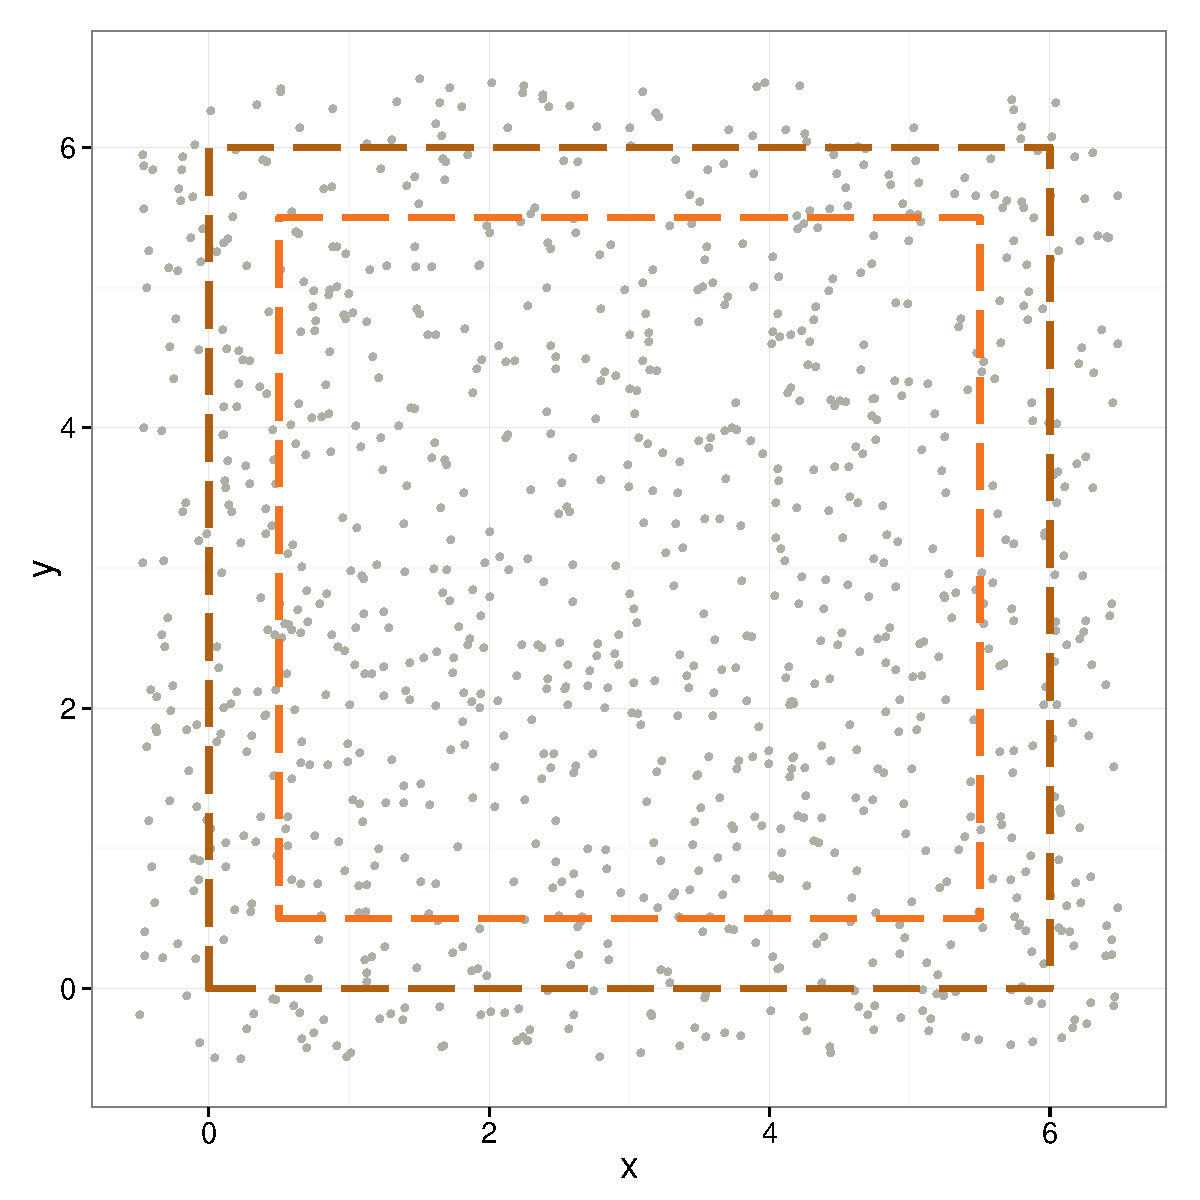
\includegraphics[height=.80\textheight]{../images/slides-pointGeneration.pdf}
	\end{figure}
\end{frame}

\begin{frame}{Half-Normal Scaling}
	The half-normal parameter $\theta$ is related to the standard deviation of a standard normal distribution by the relationship: 
	\begin{center}
	$\theta = \dfrac{\sqrt{\pi /2}}{\sigma}$
	\end{center}
	
	
	If we estimate $\sigma$ by $w/3.5$ (with $w$ being the maximum distance at which we might observe an object, and 3.5 being the standard deviation point where $P(X > 3.5) < 0.001$) then $\theta$ is:
	\begin{center}
	$\sigma = \dfrac{w}{3.5} = 0.1429$\\
	\vspace{0.5cm}
	$\theta = \dfrac{\sqrt{\pi /2}}{0.1429}=8.7732$
	\end{center}
\end{frame}

\begin{frame}{Half-Normal Scaling}
	For a half-normal with parameter $\theta=8.7732$, $f(0)=5.5852$ so to scale the value to 1:
	\begin{center}
	$\delta_{HN} = \dfrac{1}{5.5852} = 0.1790$
	\end{center}
	
	
	Half-normal density functions were executed in R with the \texttt{fdrtool} package.
\end{frame}

\end{document}